%!TEX root = ../proyecto.tex
\section{CUDA.}
Como comentábamos al principio, \cuda \textit{(Computer Unified Device Arquitecture)} \cite{cuda} es una tecnología propietaria desarrollada por \textit{NVIDIA} y lanzada en junio de 2007, que nos proporciona de un lenguaje de programación general destinado a ser ejecutado en las tarjetas gráficas de la compañía. Para los propósitos de este trabajo y, habitualmente, a la hora de trabajar con \cuda denominaremos como \textbf{\textit{host}} a la CPU que se comunica con la tarjeta gráfica y como \textbf{dispositivo} a la GPU o tarjeta gráfica utilizada. \\

La intercomunicación entre \textit{host} y dispositivo sigue un modelo maestro-esclavo. El \textit{host} actúa como maestro y es el encargado de indicar al dispositivo el código que ha de ejecutar y mandar el trabajo al dispositivo. Además, el \textit{host} tiene la posibilidad de trabajar de forma asíncrona con la GPU mientras la cola de trabajos del dispositivo no esté llena.\\

Es de vital importancia a la hora de trabajar con la GPU de tener en cuenta que:\\
\begin{itemize}
    \item a) La GPU tiene muchos más núcleos \textit{(cores)} que una CPU, lo que nos permite realizar mucha más operaciones en el mismo instante. Sin embargo, esto viene a expensas de un menor número de operaciones por segundo de cada núcleo, ya que para disfrutar de la cantidad masiva de núcleos que tiene una GPU es necesario que ésta opere a una frecuencia más baja.

    \item b) La GPU tiene su propia estructura de memoria, que ha de usar para poder realizar operaciones. Dentro de la jerarquía de memoria encontramos memoria RAM similar a la que utiliza la CPU a través de la placa base, así como varios niveles de caché. Además, hemos de tener en cuenta que a la hora de ejecutar algo en la GPU vamos a tener un gasto extra de tiempo por el traspaso de información de CPU a GPU y viceversa. Minimizar la información que ha de traspasarse en ambos sentidos así como intentar que toda la información necesaria sea transferida a la vez para sacar máximo potencial del PCI Express y exprimir al máximo posible el uso eficiente de la memoria caché, que en \cuda es habitualmente realizado mediante el manejo de la ``memoria compartida'' es fundamental para obtener mejores resultados, especialmente, aquellos en los que el cuello de botella es la transferencia de datos.

    \item c) Como la GPU tiene su propia memoria dedicada de un tamaño limitado hemos de hacer hincapié en no utilizar soluciones que generan demasiada complejidad espacial, ya que limitan la escalabilidad de los algoritmos.
\end{itemize}

\subsection{Python, NumPy, Numba y CuPy.}
Para desarrollar el código asociado a este proyecto, hemos optado por utilizar \textbf{Python} en vez de los tradicionales C o C++. El uso de \textit{Python} nos permite un desarrollo de los algoritmos más rápido así como el acceso a abstracciones de más alto nivel mediante el uso de la librerías \textbf{\textit{Numba}} y \textbf{\textit{NumPy}},  así como una mayor facilidad para la distribución del código, si se desea, mediante el uso de \textit{PyPI(Python Package Index)}, el repositorio de paquetes para Python. \\

\textbf{NumPy} \cite{numpy} es un paquete de código abierto para Python diseñado para la computación científica. El paquete proporciona una potente estructura de datos para trabajar con arrays N-dimensionales y herramientas para realizar una gran cantidad de operaciones sobre los mismos (operaciones de cálculo matricial, algoritmos de álgebra lineal y generación de números pseudoaleatorios, entre otros).\\

\textbf{Numba} \cite{numba} es un paquete para Python, cuyo objetivo es la aceleración compilando fragmentos de código con el compilador LLVM y, dando la oportunidad de paralelizar código, tanto para la CPU como para la GPU. En concreto, para las GPUs CUDA, proporciona al usuario un subconjunto de las características de CUDA con un nivel de abstracción mayor. Con eso, no sólo conseguimos poder trabajar con CUDA desde Python sino, también evitar, si lo deseamos, manejar las transferencias de memoria entre \textit{host} y dispositivo o la necesidad de indicar todos los tipos a la hora de inicializar un \textit{kernel} entre otras ventajas.\\

\textbf{CuPy} \cite{cupy} es otro paquete de Python que, por un lado y, de manera similar a Numba, nos permite generar kernels de manera similar a los de C/C++, así como facilidades para generar kernels en los que se implementa reducciones u operaciones elemento a elemento en un array. Además, CuPy está implementado de manera que permite utilizar directamente sus estructuras de datos sobre kernels de Numba, lo que nos permite combinar elementos de ambos paquetes según nos interese. \\

Por otro lado, proporciona una API similar a la de NumPy, pero las operaciones están implementadas utilizando CUDA y, tienen algunas diferencias notables entre sí, como que: el generador de pseudoaleatorios de CuPy sólo puede usar un valor escalar y, el de NumPy, puede usar también un array con múltiples valores para generar más entropía; utilizar índices por encima del tamaño de un array genera un error en NumPy pero, en CuPy, vuelve a recorrer el array desde el principio; o que, mientras que en NumPy puedes utilizar objetos de Python, en CuPy sólo puedes usar tipos de datos numéricos y booleanos.\\

\subsection{Estructura de hebras, bloques y mallas.}
El \textbf{\textit{kernel}} es un fragmento de código especial, destino a ser ejecutado en el dispositivo, en el que se indica las instrucciones que ha de ejecutar una hebra.\\
\begin{code}
\begin{minted}[fontsize=\footnotesize]{python}
from numba import cuda
import numpy as np
# Definimos el kernel
@cuda.jit
def aumentar_en_1(un_array):
  # Cogemos el índice de la hebra
    pos = cuda.grid(1)
    # Si el índice está en el rango del array
    # incrementamos su valor
    if pos < un_array.size:
        un_array[pos] += 1

if __name__ == '__main__':
  # Declaramos un array de 10000 ceros
  ejemplo = np.zeros(10000)
  # Optamos por 128 hebras por bloque
  tpb = 128
  # Calculamos el número de bloques necesario
  bloques = ejemplo.size // tpb + 1
  # Lanzamos el kernel con bloques de 128 hebras
  aumentar_en_1[bloques, tpb](ejemplo)
\end{minted}
\captionof{listing}{Kernel para incrementar en 1 los elementos de un array.\\\\}
\label{code:numbaexample}
\end{code}

Las \textbf{hebras} son la unidad mínima en la arquitectura \cudanospace. Cada hebra es ejecutada por un núcleo \cuda y es consciente, en tiempo de ejecución, de su identificador dentro del bloque así como del identificador del bloque en el que se encuentra y el tamaño del mismo, permitiéndonos así repartir el trabajo en función de dichos valores.\\

El \textbf{bloque} se corresponde a un conjunto de hebras que ejecuta el mismo \textit{kernel} y pueden cooperar entre sí. Al conjunto de esos bloques, se le denomina \textbf{``grid'' o malla}. \\

Tanto las hebras dentro de un bloque, como los bloques dentro de una malla, pueden tener estructuras unidimensionales, bidimensionales y tridimensionales. Las dimensiones de estas estructuras será indicada por el \textit{host} a la hora de ejecutar el \textit{kernel}.\\

\begin{table}[ht]
\centering
\begin{tabular}{@{}ll@{}}
\toprule
\textbf{Variable}                            & \textbf{Significado}                        \\ \midrule
\textit{\textbf{cuda.threadIdx.{[}x\textbar y\textbar z{]}}} & Índice de la hebra dentro del bloque        \\
\textit{\textbf{cuda.blockDim.{[}x\textbar y\textbar z{]}}} & Número de hebras en el bloque.              \\
\textit{\textbf{cuda.blockIdx.{[}x\textbar y\textbar z{]}}}  & Índice del bloque dentro del grid.          \\
\textit{\textbf{cuda.gridDim.{[}x\textbar y\textbar z{]}}}   & Número de bloques en el grid.               \\
\textit{\textbf{cuda.grid()}}                & Identificador único de la hebra en el grid. \\
\textit{\textbf{cuda.gridsize()}}            & Número total de hebras que usa el grid.     \\ \bottomrule
\end{tabular}
\caption{Variables para indexación de hebras con Numba CUDA.}
\label{tab:blockscuda}
\end{table}

\cuda exige que un mínimo de 32 hebras, denominado \textit{warp}, ejecuten instrucciones a la vez, aunque se hagan cálculos innecesarios así como que todas las hebras de un bloque sean ejecutadas por el mismo \textit{Streaming MultiProcessor}, de ahora en adelante, SM, que es uno de los procesadores en el dispositivo y dispone de un número específico de núcleos \cudanospace, sus propios registros y su propia caché, entre otros.\\

\begin{figure}[ht]
\centering
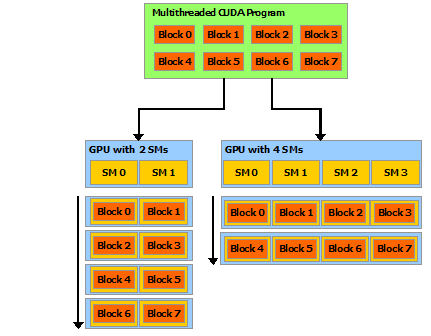
\includegraphics[scale=1.0]{imagenes/blocks.png}
\caption{Distribución de bloques de un kernel en SMs.}
\label{img:cudablocks}
\end{figure}

Al lanzar un \textit{kernel} hemos de utilizar al menos un bloque de $N$ hebras. Además, en los casos unidimensionales, el número de hebras por bloque está limitado a un máximo que depende de la tarjeta gráfica en cuestión, habitualmente 1024 hebras. No obstante, ni el uso de un único bloque de N hebras ni N bloques de 1 hebra es recomendable, ya que estaríamos dejando gran parte de la capacidad de computación paralela del dispositivo \cuda sin ser usada. En el primer caso, al haber un único bloque, sólo estaríamos haciendo uso de uno de los múltiples SMs que nos ofrece el dispositivo CUDA; en el segundo caso, al tener cada bloque una hebra, dado que los hebras de un bloque se ejecutan en \textit{warps}, cada bloque usaría 1 de las 32 hebras disponibles. 


\subsection{Estructura de memoria y memoria compartida.}
Dentro de la tarjeta gráfica, nos encontramos con distintos niveles de memoria. Una vez los datos necesarios han sido traspasados del \textit{host} al dispositivo a través del bus PCI Express, esos datos son almacenados en una memoria DRAM de propósito general del dispositivo. Cuando un \textit{kernel} solicita datos de esta memoria, de manera similar a como ocurre en una CPU, los datos solicitados y los colindantes en memoria son colocados a través de varios niveles de caché, que tiene tamaño más limitado que la memoria DRAM pero con un acceso de lectura y escritura mucho más rápido.\\

\begin{table}[H]
\centering
\begin{tabular}{@{}cccc@{}}
\toprule
\textbf{\textbf{Memoria}} & \textbf{\textbf{Localización}}                                  & \textbf{\begin{tabular}[c]{@{}c@{}}Acceso\\ (E = Escribir)\\ (L = Leer)\end{tabular}} & \textbf{\begin{tabular}[c]{@{}c@{}}Existente\\ hasta fin\\ de\end{tabular}} \\ \midrule
\textbf{Registro}         & Caché                                                           & Kernel (E/L)                                                                          & Hebra                                                                       \\
\textbf{Local}            & \begin{tabular}[c]{@{}c@{}}DRAM\\ (Caché tras uso)\end{tabular} & Kernel (E/L)                                                                          & Hebra                                                                       \\
\textbf{Compartida}       & Caché                                                           & Kernel (E/L)                                                                          & Bloque                                                                      \\
\textbf{Global}           & \begin{tabular}[c]{@{}c@{}}DRAM\\ (Caché tras uso)\end{tabular} & \begin{tabular}[c]{@{}c@{}}Host (E/L)\\ Kernel (E/L)\end{tabular}                     & \begin{tabular}[c]{@{}c@{}}Aplicación\\ o uso de free\end{tabular}          \\
\textbf{Constante}        & \begin{tabular}[c]{@{}c@{}}DRAM\\ (Caché tras uso)\end{tabular} & \begin{tabular}[c]{@{}c@{}}Host (E/L)\\ Kernel (L)\end{tabular}                       & \begin{tabular}[c]{@{}c@{}}Aplicación \\ o uso de free\end{tabular}         \\ \bottomrule
\end{tabular}
\caption{Resumen de los tipos de memoria en CUDA.}
\label{tab:cudamemory}
\end{table}


La \textbf{memoria compartida} es una abstracción para una región especial de la caché asociada a un bloque que es explícitamente usada por el programador en el \textit{kernel}, agilizando así considerablemente las transferencias de memoria en el dispositivo. En el cuadro \ref{tab:cudamemory}, podemos ver un resumen de los tipos de memoria existentes, dónde se pueden usar y dónde se encuentran dichos datos en el dispositivo.\\


Si utilizamos los arrays N-dimensionales de NumPy, no tenemos la necesidad de realizar las transferencias de memoria. No obstante, es recomendable manejarlas manualmente para evitar cualquier transferencia de datos entre \textit{host} y dispositivo innecesaria. 

\begin{table}[ht]
\begin{tabular}{@{}ll@{}}
\toprule
\textbf{Función}                                                                                                          & \textbf{Definición}                                                                                                                                            \\ \midrule
\textbf{\begin{tabular}[c]{@{}l@{}}cuda.device\_array(dimensiones,\\                                  tipo)\end{tabular}} & \begin{tabular}[c]{@{}l@{}}Declara un array con las dimensiones \\ y tipo de datos dados en memoria \\ global. Invocada desde \textit{host}.\end{tabular}      \\ \midrule
\textbf{cuda.to\_device(array)}                                                                                           & \begin{tabular}[c]{@{}l@{}}Envía array de la memoria del \textit{host} \\ a la memoria global del \\ dispositivo. Invocada desde \textit{host}.\end{tabular}   \\ \midrule
\textbf{d\_array.copy\_to\_host()}                                                                                        & \begin{tabular}[c]{@{}l@{}}Método para enviar d\_array de la \\ memoria del dispositivo a la del \\ \textit{host}. Invocada desde \textit{host}.\end{tabular}  \\ \midrule
\textbf{\begin{tabular}[c]{@{}l@{}}cuda.local.array(dimensiones,\\                              tipo)\end{tabular}}       & \begin{tabular}[c]{@{}l@{}}Declara un array con las dimensiones\\ y tipo de datos dados en memoria \\ local. Invocada desde \textit{kernel}.\end{tabular}      \\ \midrule
\textbf{\begin{tabular}[c]{@{}l@{}}cuda.shared.array(dimensiones,\\                                  tipo)\end{tabular}}  & \begin{tabular}[c]{@{}l@{}}Declara un array con las dimensiones\\ y tipo de datos dados en memoria \\ compartida. Invocada desde \textit{kernel}.\end{tabular} \\ \bottomrule
\end{tabular}
\caption{Algunas funciones para trabajar con la memoria del dispositivo en CUDA.}
\label{tab:cudamemoryfuncs}
\end{table}

\subsection{Sincronización y operaciones atómicas.}
Es frecuente la necesidad de que múltiples hebras cooperen, usando datos en alguna región de memoria del dispositivo, a la que tienen acceso de forma simultánea. En estos casos, podríamos encontrarnos ante el riesgo de una dependencia de datos de tipo \textit{RAW (Read After Write)}, es decir, una situación en la que se lee un dato antes de que los cálculos previos que necesitamos se hayan realizado. Para evitar este tipo de dependencias, \cuda proporciona varios mecanismos para sincronizar las hebras usadas, de los que vamos a destacar los dos usados en este trabajo.\\

Por un lado, si no estamos utilizando los \textit{streams} de \cudanospace, característica que permite lanzar \textit{kernels} distintos de forma concurrente, tenemos garantizado que un \textit{kernel} no será ejecutado hasta que el \textit{kernel} anterior no haya terminado de procesarse. El uso de múltiples \textit{kernels} no es recomendable si no es necesario, ya que, cuando queden pocas operaciones por realizar en uno de los \textit{kernels}, parte del dispositivo podría no estar realizando cálculo alguno, y, en el lanzamiento de cada \textit{kernel}, existe un pequeño intervalo de tiempo desde que el \textit{host} invoca el \textit{kernel} y éste empieza a ser ejecutado en la GPU.\\ 

Por otro lado, dentro de un bloque, podemos sincronizar todas las hebras del mismo mediante el uso de la función \textbf{\textit{cuda.syncthreads()}}. Esta función, que es invocada desde un \textit{kernel}, garantiza que todas las instrucciones hasta el punto de invocación han sido ejecutadas por todas las hebras del bloque. Para ello, las hebras que ya han realizado los cálculos se quedan esperando a que las otras terminen, por lo que sólo debe usarse cuando sea necesario.\\


Otra forma de evitar los riesgos \textit{RAW} es el uso de operaciones atómicas. Las operaciones atómicas son instrucciones que realizan la lectura, modificación y escritura de una posición de memoria global o compartida a la vez, es decir, está garantizado que realice todas sus operaciones antes de que otra hebra trabaje sobre la misma posición de memoria. Imaginemos el caso en el que una posición de memoria tiene un valor, 0, y dos hebras, A y B, quieren sumar dos valores: 1 y 2, respectivamente. El resultado final que deberíamos obtener sería 3, sin embargo, si no usamos las operaciones atómicas podría ocurrir que: en primer lugar, las hebras A y B leen el valor 0; en segundo lugar, A suma 1 y lo escribe en la posición de memoria; por último, B suma 2 a lo que había leído (0), con lo que en la posición de memoria queda como resultado final 2. El uso de las operaciones atómicas asegura que estas situaciones no ocurran a cambio de que la operación sea más lenta que una suma tradicional, especialmente cuando muchas hebras quieren modificar la misma posición de memoria. La suma atómica es utilizada en Numba con la función \textbf{\textit{cuda.atomic.add(my\_array, posición, valor\_a\_sumar)}}.


\subsection{Generación de números pseudoaleatorios en la GPU.}

\textit{Numba} nos proporciona un generador de números pseudoaleatorios para \cudanospace, utilizando el algoritmo \textit{xoroshiro128+} \cite{xoroshiro}, para generar números de una distribución uniforme y, el método de Box-Muller, para transformar la distribución uniforme a una distribución normal.\\

En la GPU, para que el generador pueda ser inicializado con una semilla, ha de generarse un estado aleatorio para cada hebra, ya que, si todas las hebras usaran el mismo, el orden en el que se ejecuten las hebras afectaría al resultado. Por ello, Numba nos proporciona la función \textbf{create\_xoroshiro128p\_states(n, seed)}, que se invoca desde el \textit{host} devuelve un array en la memoria global del dispositivo con los estados aleatorios para $n$ hebras basados en la semilla $seed$.\\

La función \textbf{xoroshiro128p\_[distribución]\_[tipo](estados, id\_hebra)}, invocada desde el \textit{kernel}, nos permite obtener números pseudoaleatorios de la distribución y tipo proporcionados. La distribución puede ser: \textit{uniform}, para la distribución uniforme; y \textit{normal}, para una distribución normal. Los dos tipos de datos soportados son valores en coma flotante de 32 bits \textit{(float32)} o valores en coma flotante de 64 bits \textit{(float64)}. \\

\begin{code}
\begin{minted}{python}
from numba.cuda.random import create_xoroshiro128p_states
from numba.cuda.random import xoroshiro128p_uniform_float32
import numpy as np
@cuda.jit
def pseudoaleatorios(rng_states, array):
    """
    :param rng_states Estados aleatorios.
    :param array Array a inicializar
    """
    # La hebra coge su identificador unidimensional único.
    idx = cuda.grid(1)

    # Sacamos el float32 aleatorio correspondiente.
    if idx < array.size:
        array[idx] = xoroshiro128p_uniform_float32(rng_states,
                                                   idx)

# Tamaño del array
n = 10000
# Generamos un array de flot32 sin inicializar.
mi_array = np.empty(n, dtype=np.float32)
# Generamos los estados aleatorio de todas las hebras para la semilla 7.
rng_states = create_xoroshiro128p_states(n, seed=7)
# Número de hebras por bloque
tpb = 512
# Invocamos el kernel para inicializar mi_array con pseudoaleatorios.
pseudoaleatorios[mi_array.size // tpb + 1, tpb](rng_states, mi_array)
\end{minted}
\captionof{listing}{Inicialización pseudoaleatoria de un array.\\}
\label{code:randoms}
\end{code}

\subsection{Streams.}
Un \textbf{stream} en \textit{CUDA} es una secuencia de órdenes (lanzamiento de \textit{kernels}, transferencias de memoria, etc.) enviadas desde el \textit{host} al dispositivo. Mientras que la secuencia de órdenes dentro de un \textit{stream} ha de ser ejecutada secuencialmente, las órdenes entre los \textit{streams} pueden intercalarse, potencialmente permitiendo un mejor uso de los recursos al ejecutar múltiples \textit{kernels} de forma concurrente. \\

\textit{Numba} nos permite utilizar esta característica con la función \textbf{cuda.stream()}, que genera un nuevo stream y nos devuelve el identificador del mismo. Para usarlo, al lanzar el kernel o hacer la transferencia de memoria hemos de pasar la variable con el identificador en el parámetro posicional ``stream'. Posteriormente, podemos sincronizar todos los \textit{streams} utilizando la función \textbf{cuda.synchronize()}. \\

\begin{code}
\begin{minted}{python}
...
# Generamos dos streams
stream1 = cuda.stream()
stream2 = cuda.stream()

# Declaramos dos arrays de 100000 elementos
n = 100000 
array1 = np.ones(n, dtype=np.float32)
array2 = np.empty(n, dtype=np.float32)

# Hacemos las transferencias de memoria
d_array1 = cuda.to_device(array1, stream=stream1)
d_array2 = cuda.to_device(array2, stream=stream2)

tpb = 128
bloques = n // tpb + 1

# Lanzamos los kernels de forma asíncrona usando
# los straems
aumentar_en_1[bloques, tpb, stream1](d_array1)
rng_states = create_xoroshiro128p_states(n, seed=7)
pseudoaleatorios[bloques, tpb, stream2](rng_states, d_array2)

# Traemos de vuelta los arrays al host
array1 = d_array1.copy_to_host(stream=stream1)
array2 = d_array2.copy_to_host(stream=stream2)

# Sincronizamos para asegurar que ambos streams han finalizado.
cuda.synchronize()
\end{minted}
\captionof{listing}{Uso de streams en CUDA para ejecución concurrente.\\}
\label{code:streams}
\end{code}

\section{Spark.}



\textbf{\textit{Apache Spark}} es un \textit{framework} de código abierto y propósito general para sistemas distribuidos de computación en clúster, que proporciona una API utilizable desde los lenguajes de programación en Scala, Java, Python y R; y proporciona herramientas de alto nivel como ML/MLib, una librería con algoritmos de \textit{machine learning}. \\

El \textit{framework} fundamenta su arquitectura en el \textit{RDD (Resilient Distributed DataSet)}, que es una estructura de datos de sólo lectura distribuida en un clúster de máquinas, mantenida durante toda la computación y con tolerancia a fallos. El hecho de que el RDD sea inmutable, es decir, de sólo lectura, facilita la distribución del trabajo a lo largo del clúster aunque implica que las acciones que transforman los datos, necesiten crear un nuevo \textit{RDD} para los resultados. Existen dos formas básicas de generar un \textit{RDD} en \textit{Spark}: paralelizando una colección existente en el código que controla la ejecución de \textit{Spark} o leyendo los datos de un sistema de almacenamiento. \\

Al poder utilizar la \textit{API} desde \textit{Python} podemos combinar de una manera simple el uso de \textit{Spark} y \textit{CUDA}. El uso de ambas nos proporcion, entre otras, las siguientes ventajas:\\

\begin{itemize}
  \item \textit{Spark} nos proporciona herramientas para la lectura de datos desde un sistema de almacenamiento.
  \item El código que realicemos combinando \textit{Spark} y \textit{CUDA} podría ser usado tanto en una única máquina como en un clúster.
  \item Si trabajamos con una única máquina, podemos solucionar problemas de escalabilidad ajustando el número de particiones (subdivisiones del RDD) y el número de ejecutores (número de procesos que podrían ejecutarse simultáneamente) para, por ejemplo, evitar quedarnos sin memoria \textit{RAM} en el dispositivo.\\
\end{itemize}

La distribución de trabajo en Spark en este proyecto se realizará utilizando la transformación \textit{mapPartitions} del \textit{RDD}, que generará un nuevo RDD a partir de los resultados obtenidos al aplicar la función pasada a \textit{mapPartitions} como parámetro a cada una de las funciones. \\

\begin{code}
\begin{minted}{python}
import numpy as np
from pyspark.sql import SparkSession

# Cogemos el contexto de Spark
spark = SparkSession.builder.master("local").appName("ejemplo").getOrCreate()
sc = spark.sparkContext

# Generamos un array de 100000 ceros.
mi_array = np.zeros(100000, np.float32)

# Creamos un RDD a partir del array
rdd = sc.parallelize(mi_array)

# Número de hebras por bloque
tpb = 128

# Encapsulamos un kernel en una función de Python
def gpu_work(data):
  # Transformamos los datos a un array de NumPy
  gpu_data = np.asarray(list(data), dtype=np.float32)
  # Invocamos el kernel utilizado en los ejemplos previos.
  aumentar_en_1[gpu_data.size // tpb + 1, tpb](gpu_data)
  # Devolvemos los datos calculados
  return gpu_data


# Realizamos la transformación del RDD
output = rdd.mapPartitions(gpu_work)

# Recogemos los resultados en un array de NumPy
output_np = output.collect()
\end{minted}
\captionof{listing}{Uso de Spark con Numba.\\}
\label{code:spark}
\end{code}
